\documentclass[conference]{IEEEtran}
\usepackage{amsmath,amssymb}
\usepackage{graphicx}
\usepackage{booktabs}
\usepackage{multirow}
\usepackage{url}
\usepackage{xcolor}
\usepackage{algorithm}
\usepackage{algorithmic}
\usepackage{tikz}
\usetikzlibrary{arrows.meta,positioning,fit,backgrounds}
% Same categorical palette used by the dataviz-validated Fig.~3/4 plots
% (experiments/plots/common.py's ARM_STYLE), reused here for visual
% consistency across the paper's figures.
\definecolor{palBlue}{HTML}{2A78D6}
\definecolor{palGreen}{HTML}{008300}
\definecolor{palYellow}{HTML}{EDA100}
\definecolor{palPurple}{HTML}{7A5CD6}

% Small self-contained TikZ pictograms for Fig.~2 (no external icon font/
% asset dependency) -- server rack (core), radio tower (gNB), handset (UE),
% gear (xApp/orchestrator).
\newcommand{\iconServer}[1]{\tikz[baseline=-0.55ex, scale=0.075, color=#1]{
  \foreach \i in {0,1,2} {\draw[thick] (0,\i*0.75) rectangle ++(1.9,0.55); \fill (1.6,\i*0.75+0.28) circle (0.09);}
}}
\newcommand{\iconTower}[1]{\tikz[baseline=-0.55ex, scale=0.075, color=#1]{
  \draw[thick] (-0.55,0) -- (0,1.7) -- (0.55,0);
  \draw[thick] (0,1.7) -- (0,2.0);
  \fill (0,2.05) circle (0.11);
  \draw[thick] (-0.45,2.15) -- (-0.2,1.85); \draw[thick] (0.45,2.15) -- (0.2,1.85);
  \draw[thick] (-0.75,2.4) -- (-0.35,2.0); \draw[thick] (0.75,2.4) -- (0.35,2.0);
}}
\newcommand{\iconPhone}[1]{\tikz[baseline=-0.55ex, scale=0.075, color=#1]{
  \draw[thick, rounded corners=0.15] (0,0) rectangle (1.15,2.0);
  \draw[thick] (0.3,1.65) -- (0.85,1.65);
  \draw[thick] (0.575,0.32) circle (0.16);
}}
\newcommand{\iconGear}[1]{\tikz[baseline=-0.55ex, scale=0.075, color=#1]{
  \foreach \a in {0,30,...,330} {\draw[thick] (\a:0.95) -- (\a:1.35);}
  \draw[thick] (0,0) circle (0.95);
  \draw[thick] (0,0) circle (0.4);
}}

% Visible TODO markers for content the author (not Claude) writes.
\newcommand{\authorTODO}[1]{\par\noindent\fbox{\parbox{0.95\linewidth}{\textbf{\color{red}TODO(MANOJ):} #1}}\par}
% Inline variant, safe mid-sentence: a number/figure this repo cannot verify
% and Claude must not invent (see CLAUDE.md hard constraint on TODO(MEASURE)).
\newcommand{\TODO}[1]{\textbf{\color{red}[TODO: #1]}}

% Purely typographic float-spacing tightening (no content change) --
% standard camera-ready technique to reclaim whitespace around
% figures/tables/captions.
\setlength{\textfloatsep}{5pt plus 1pt minus 2pt}
\setlength{\floatsep}{4pt plus 1pt minus 1pt}
\setlength{\intextsep}{5pt plus 1pt minus 2pt}
\setlength{\abovecaptionskip}{3pt}
\setlength{\belowcaptionskip}{0pt}
\renewcommand{\arraystretch}{0.92}

\begin{document}

\title{QoE-Aware DRL for Slice Admission Control: A Live Open RAN Testbed Validation}

\author{
\IEEEauthorblockN{Manoj Prasad Kunasegran}
\IEEEauthorblockA{School of Engineering\\Taylor's University\\Subang Jaya, Malaysia\\orcid.org/0009-0005-3169-1873}
\and
\IEEEauthorblockN{Wai Leong Pang*}
\IEEEauthorblockA{School of Engineering\\Taylor's University\\Subang Jaya, Malaysia\\orcid.org/0000-0001-8407-5648\\*Corresponding author}
\and
\IEEEauthorblockN{Swee King Phang}
\IEEEauthorblockA{School of Engineering\\Taylor's University\\Subang Jaya, Malaysia\\orcid.org/0000-0002-7877-8766}
}

\maketitle

\begin{abstract}
Building on our previous work on Deep Reinforcement Learning
(DRL)-driven Slice Admission Control (SAC), validated entirely in
simulation, this paper moves the same control problem onto a real
Open RAN testbed. We deploy a Quality of Experience (QoE)-aware Deep
Q-Network (DQN) admission policy on a real OpenAirInterface (OAI)
gNodeB (gNB) across three network slices (eMBB, URLLC, mMTC) and
compare it against a static baseline and a best-possible
static-at-cap policy. After identifying and correcting a calibration
issue in our QoE estimation, a fully powered live re-evaluation (128
episodes per arm) shows DQN under the QoE-aware reward sustaining
100\% SLA compliance throughout, significantly ahead of the static
baseline (Fisher exact $p=0.0070$, $p=0.0209$ after Holm-Bonferroni
correction across the family of arm-vs-baseline comparisons) --
our clearest evidence yet that a QoE-aware learned policy outperforms
static control on real hardware. Honest limits accompany that result:
the SLA-only reward and the static-at-cap arm converge to a
statistically indistinguishable rate (126 of 128 episodes fully
compliant for each, Fisher exact $p=1.0$) that remains only
numerically, not significantly, above the static baseline's 120 of
128 -- the collapse-avoidance edge our earlier, smaller-sample
evaluation suggested for the SLA-only reward does not hold at this
larger, well-powered scale. Checking five further
independently-trained SLA-reward checkpoints, at a reduced 21-episode
protocol, shows live robustness varies substantially by training seed
despite equivalent offline convergence, which we trace in part to the
offline training environment's own fidelity to real traffic dynamics.
We additionally live-evaluate checkpoints trained for a congested,
URLLC-preservation scenario: unlike its offline counterpart, where
DQN measurably trades eMBB compliance for URLLC under an imposed
shared-resource-pool constraint, every arm is fully SLA-compliant
live, since this rig's calibrated ceilings are too small relative to
the gNB's real capacity for the same forced scarcity to arise --
though, at this pilot scale (one seed, two episodes/arm), the
QoE-aware reward still yields a materially higher URLLC Mean Opinion
Score at the same compliance level. We also report the control-loop
latency and model footprint needed for practical deployment. These
findings demonstrate the feasibility, and surface the honest limits,
of deploying DRL-driven SAC on real Open RAN hardware.
\end{abstract}

\begin{IEEEkeywords}
5G, Network Slicing, Slice Admission Control, Deep Reinforcement Learning, Quality of Experience, Open RAN
\end{IEEEkeywords}

\section{Introduction and Background}
Network slicing (NS) lets a single physical 5G deployment serve
heterogeneous service classes under per-slice Service Level
Agreements (SLAs): Ultra-Reliable Low-Latency Communication (URLLC)
requires sub-millisecond latency and high reliability, Enhanced
Mobile Broadband (eMBB) demands high throughput, and Massive
Machine-Type Communication (mMTC) accommodates large numbers of
low-power devices. Slice Admission Control (SAC) decides whether an
incoming slice request can be accommodated given current resource
availability. Static, threshold-based SAC cannot adapt its
allocation as demand shifts, motivating context-aware, learning-based
approaches.

Our prior work applied Deep Reinforcement Learning (DRL) to SAC
under gNodeB (gNB) congestion, using SLA-driven reward shaping to
prioritise URLLC traffic, and later extended this to a third slice
(mMTC) with a load-balancing objective across multiple gNBs
\cite{mecon-paper1,icraie-paper2}. Both studies sat in the
simulation-only evidence tier that our systematic review of the
2024--2026 literature identifies as covering
\TODO{sim-only fraction from [3] evidence tiers} of DRL-driven SAC work
surveyed there \cite{survey-paper3}; that same evidence-tier analysis
finds the live-hardware tier for this formulation unoccupied. This
paper closes that gap: we realise the same admission-control problem
on a real OAI gNB over its native E2 control interface, with the radio
channel still simulated (rfsim), occupying the tier
\cite{survey-paper3} identifies as missing, and centre the evaluation
on Quality of Experience (QoE) rather than SLA compliance alone.

This paper makes the following contributions:
\begin{enumerate}
\item We deploy a DRL-based SAC policy on a real O-RAN E2 control
loop and identify a structural difference from our earlier simulated
work: the real E2 interface exposes no per-flow accept/reject
primitive, only a per-slice resource ceiling, so admission must be
realised as an adjustment of that ceiling.
\item We compare a QoE-aware reward directly against the SLA-only
reward of \cite{mecon-paper1,icraie-paper2} on the same live
hardware.
\item We add a static-at-cap arm that isolates whether the learned
policy's advantage is genuine admission timing, or simply the result
of using a more generous static allocation.
\item We report the engineering numbers (control-loop latency, model
size) a real deployment needs, a calibration issue found and fixed in
our QoE estimation, and the fully powered re-evaluation that
correction enabled.
\item We evaluate a congested, multi-slice traffic scenario both
offline and, at a smaller scale, live, showing where the offline
scarcity mechanism does and does not carry over to real hardware.
\item We show that live robustness varies substantially across
independently-trained checkpoints despite equivalent offline
convergence, and identify a corresponding limitation in the offline
training environment itself.
\item This single-agent, single-gNB deployment is a deliberate reduced
case of our systematic review's proposed graph-attention, multi-agent,
federated-learning (GAT-MARL-FL) framework \cite{survey-paper3}: it
validates, on real hardware, the control loop that fuller architecture
would sit on top of.
\end{enumerate}

The remainder of this paper is organised as follows: Section II
reviews related work on DRL-driven SAC. Section III describes the
live testbed, the problem formulation, and the reward function.
Section IV presents and discusses the results. Section V concludes
the paper and outlines future work.

\section{Literature Review}
\authorTODO{Literature review to be added here, following the style
of Section II in our prior conference papers~\cite{mecon-paper1,icraie-paper2}
(narrative summary of $\sim$10--12 related DRL-driven SAC / real-testbed
studies, each introduced with ``The authors in [X] proposed...''),
concluding with a short paragraph positioning this paper against that
related work. Candidate sources are already screened in our
systematic review~\cite{survey-paper3}.}

\section{Methodology}
Fig.~\ref{fig:pipeline} summarises the pipeline detailed in this
section: offline training against a closed-loop simulator
(Section~III-C) produces frozen checkpoints, deployed on the live
testbed below with no further learning, and evaluated both live and,
separately, offline against fresh held-out episodes -- a branch that,
as Section~III-C shows, does not predict the live outcome.

\begin{figure}[t]
\centering
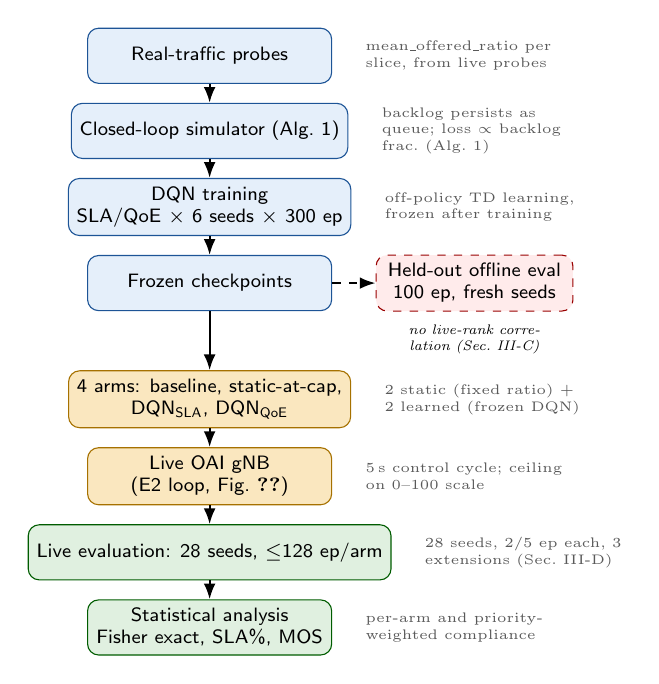
\begin{tikzpicture}[
  font=\sffamily\scriptsize,
  box/.style={draw, rounded corners, align=center, inner sep=3pt, minimum height=0.7cm, minimum width=3.1cm},
  simbox/.style={box, fill=palBlue!12, draw=palBlue!70!black},
  livebox/.style={box, fill=palYellow!25, draw=palYellow!70!black},
  evalbox/.style={box, fill=palGreen!12, draw=palGreen!70!black},
  warnbox/.style={box, fill=red!8, draw=red!60!black, dashed, minimum width=2.5cm},
  arrow/.style={-{Latex[length=2mm]}, thick},
  dashedarrow/.style={-{Latex[length=2mm]}, thick, dashed},
]
\node[simbox] (probe) {Real-traffic probes};
\node[simbox, below=0.24cm of probe] (sim) {Closed-loop simulator (Alg.~1)};
\node[simbox, below=0.24cm of sim] (train) {DQN training\\SLA/QoE $\times$ 6 seeds $\times$ 300 ep};
\node[simbox, below=0.24cm of train] (ckpt) {Frozen checkpoints};
\node[livebox, below=0.75cm of ckpt] (arms) {4 arms: baseline, static-at-cap,\\DQN$_{\text{SLA}}$, DQN$_{\text{QoE}}$};
\node[livebox, below=0.24cm of arms] (rig) {Live OAI gNB\\(E2 loop, Fig.~\ref{fig:architecture})};
\node[evalbox, below=0.24cm of rig] (liveeval) {Live evaluation: 28 seeds, $\leq$128 ep/arm};
\node[evalbox, below=0.24cm of liveeval] (stats) {Statistical analysis\\Fisher exact, SLA\%, MOS};

\draw[arrow] (probe) -- (sim);
\draw[arrow] (sim) -- (train);
\draw[arrow] (train) -- (ckpt);
\draw[arrow] (ckpt) -- (arms);
\draw[arrow] (arms) -- (rig);
\draw[arrow] (rig) -- (liveeval);
\draw[arrow] (liveeval) -- (stats);

% Side annotations -- fill the whitespace beside the main chain with the
% concrete detail each stage's prose already states, instead of leaving
% it empty.
\node[font=\tiny, text=black!65, align=left, text width=2.5cm, anchor=west] at ([xshift=0.3cm]probe.east) {mean\_offered\_ratio per slice, from live probes};
\node[font=\tiny, text=black!65, align=left, text width=2.5cm, anchor=west] at ([xshift=0.3cm]sim.east) {backlog persists as queue; loss $\propto$ backlog frac.\ (Alg.~1)};
\node[font=\tiny, text=black!65, align=left, text width=2.5cm, anchor=west] at ([xshift=0.3cm]train.east) {off-policy TD learning, frozen after training};
\node[font=\tiny, text=black!65, align=left, text width=2.5cm, anchor=west] at ([xshift=0.3cm]arms.east) {2 static (fixed ratio) + 2 learned (frozen DQN)};
\node[font=\tiny, text=black!65, align=left, text width=2.5cm, anchor=west] at ([xshift=0.3cm]rig.east) {5\,s control cycle; ceiling on 0--100 scale};
\node[font=\tiny, text=black!65, align=left, text width=2.5cm, anchor=west] at ([xshift=0.3cm]liveeval.east) {28 seeds, 2/5 ep each, 3 extensions (Sec.~III-D)};
\node[font=\tiny, text=black!65, align=left, text width=2.5cm, anchor=west] at ([xshift=0.3cm]stats.east) {per-arm and priority-weighted compliance};

\node[warnbox, right=0.55cm of ckpt] (offeval) {Held-out offline eval\\100 ep, fresh seeds};
\draw[dashedarrow] (ckpt.east) -- (offeval.west);
\node[font=\tiny\itshape, below=0.04cm of offeval, align=center, text width=3.0cm] {no live-rank correlation (Sec.~III-C)};
\end{tikzpicture}
\caption{End-to-end methodology. Real-traffic probe measurements calibrate the offline simulator (Section~III-C, Algorithm~1); DQN training produces frozen checkpoints for both reward variants, joined by the two static arms into the four compared conditions, deployed live with no further learning; live episodes are logged and reduced to Table~\ref{tab:results}/Figs.~\ref{fig:compliance}--\ref{fig:ceiling} via Fisher exact tests and MOS. A held-out offline evaluation runs alongside this live pipeline but, per Section~III-C, does not predict its outcome.}
\label{fig:pipeline}
\end{figure}

\subsection{Testbed}
Fig.~\ref{fig:architecture} shows the resulting software architecture:
an Open5GS core, an OAI gNB enforcing per-slice ceilings, three UEs
(one per slice), and the E2 agent/xApp loop through which all four
arms issue their admission decisions.

\begin{figure*}[t]
\centering
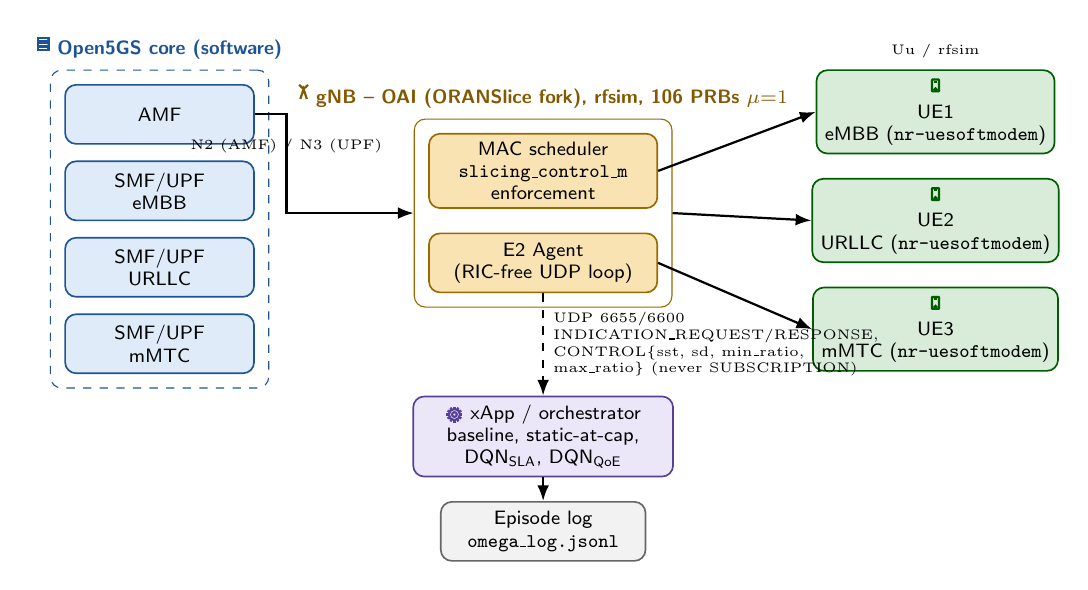
\begin{tikzpicture}[
  font=\sffamily\scriptsize,
  box/.style={draw, rounded corners, minimum height=0.75cm, align=center, inner sep=3pt, line width=0.6pt},
  core/.style={box, fill=palBlue!15, draw=palBlue!70!black},
  gnb/.style={box, fill=palYellow!30, draw=palYellow!65!black},
  ue/.style={box, fill=palGreen!15, draw=palGreen!70!black, minimum width=2.0cm},
  xapp/.style={box, fill=palPurple!15, draw=palPurple!70!black},
  logbox/.style={box, fill=black!5, draw=black!60, minimum width=2.6cm},
  arrow/.style={-{Latex[length=2mm]}, thick},
  dashedarrow/.style={-{Latex[length=2mm]}, thick, dashed},
]
\node[core, minimum width=2.4cm] (amf) {AMF};
\node[core, minimum width=2.4cm, below=0.2cm of amf] (smf1) {SMF/UPF\\eMBB};
\node[core, minimum width=2.4cm, below=0.2cm of smf1] (smf2) {SMF/UPF\\URLLC};
\node[core, minimum width=2.4cm, below=0.2cm of smf2] (smf3) {SMF/UPF\\mMTC};
\node[draw=palBlue!70!black, dashed, rounded corners, fit=(amf)(smf1)(smf2)(smf3), inner sep=5pt, label={[font=\sffamily\bfseries\scriptsize, text=palBlue!70!black]above:\iconServer{palBlue!70!black}\ Open5GS core (software)}] (core) {};

\node[gnb, minimum width=2.9cm, right=2.2cm of smf1.north east, anchor=north west, yshift=0.35cm] (mac) {MAC scheduler\\\texttt{slicing\_control\_m}\\enforcement};
\node[gnb, minimum width=2.9cm, below=0.3cm of mac] (e2) {E2 Agent\\(RIC-free UDP loop)};
\node[draw=palYellow!65!black, rounded corners, fit=(mac)(e2), inner sep=5pt, label={[font=\sffamily\bfseries\scriptsize, text=palYellow!55!black]above:\iconTower{palYellow!55!black}\ gNB -- OAI (ORANSlice fork), rfsim, 106 PRBs $\mu{=}1$}] (gnbbox) {};

\node[ue, right=2.0cm of mac, yshift=0.75cm] (ue1) {\iconPhone{palGreen!70!black}\\UE1\\eMBB (\texttt{nr-uesoftmodem})};
\node[ue, below=0.3cm of ue1] (ue2) {\iconPhone{palGreen!70!black}\\UE2\\URLLC (\texttt{nr-uesoftmodem})};
\node[ue, below=0.3cm of ue2] (ue3) {\iconPhone{palGreen!70!black}\\UE3\\mMTC (\texttt{nr-uesoftmodem})};

\node[xapp, minimum width=3.3cm, below=1.3cm of e2] (xapp) {\iconGear{palPurple!70!black}\ xApp / orchestrator\\baseline, static-at-cap,\\DQN$_{\text{SLA}}$, DQN$_{\text{QoE}}$};
\node[logbox, below=0.3cm of xapp] (log) {Episode log\\\texttt{omega\_log.jsonl}};

\draw[arrow] (amf.east) -- ++(0.4,0) coordinate (n2n3) -- (n2n3 |- gnbbox.west) node[midway, above, font=\tiny] {N2 (AMF) / N3 (UPF)} -- (gnbbox.west);
\draw[arrow] (mac.east) -- (ue1.west);
\draw[arrow] (gnbbox.east) -- (ue2.west);
\draw[arrow] (e2.east) -- (ue3.west);
\node[font=\tiny, above=0.02cm of ue1] {Uu / rfsim};
\draw[dashedarrow] (e2.south) .. controls +(0,-0.8) and +(0,0.8) .. node[right, font=\tiny, align=left] {UDP 6655/6600\\INDICATION\_REQUEST/RESPONSE,\\CONTROL\{sst, sd, min\_ratio,\\max\_ratio\} (never SUBSCRIPTION)} (xapp.north);
\draw[arrow] (xapp) -- (log);
\end{tikzpicture}
\caption{Testbed software architecture, colour-coded by component: Open5GS core (blue; AMF, per-slice SMF/UPF) over N2/N3 to an OAI gNB (yellow; ORANSlice fork, simulated radio channel, 106 PRBs at $\mu{=}1$) whose MAC scheduler enforces the per-slice ceiling; three \texttt{nr-uesoftmodem} UEs (green), one per slice, over the simulated Uu interface. The RIC-free E2 agent exchanges UDP INDICATION/RESPONSE and CONTROL (\texttt{sst}, \texttt{sd}, \texttt{min\_ratio}, \texttt{max\_ratio}) messages with the xApp/orchestrator (purple) that all four compared arms run through, which logs every step to \texttt{omega\_log.jsonl} for the offline analysis in Section~IV.}
\label{fig:architecture}
\end{figure*}

We deploy a real OAI gNB (ORANSlice fork \cite{oranslice}) with a
simulated radio channel (rfsim), an Open5GS core, and three
\texttt{nr-uesoftmodem} user equipment (UE), one per slice. The gNB
has a nominal capacity of 106 Physical Resource Blocks (PRBs, $\mu=1$
numerology). Unlike our earlier simulated work, the real O-RAN E2
interface does not expose a binary accept/reject action; its only
control primitive is a per-slice ratio ceiling on a 0--100 scale,
enforced by the MAC scheduler \cite{oran-e2ap}. We therefore realise
the admission decision as a ceiling adjustment: an accept decision
raises a slice's ceiling toward a calibrated maximum, and a reject
decision lowers it toward a floor. Ceiling values were calibrated by
direct measurement on the live rig rather than assumed, since the
0--100 ratio scale does not map linearly onto real PRBs at this
cell's configuration. The static
baseline holds its ceiling fixed for the whole episode; a second
static arm, \emph{static-at-cap}, instead pins every slice's ceiling
at its calibrated maximum from the start, isolating whether a more
generous fixed allocation alone can match a learned policy. Learned
arms are DQN policies \cite{dqn}, trained offline against a
closed-loop simulated traffic source, then evaluated live with frozen
weights.

\subsection{Problem Formulation}
The gNB state at time $t$ is defined as
\begin{equation}
s_t = \left(\frac{U_s(t)}{B}, \; C_t, \; \frac{L_s(t)}{L_{\max}} \;\forall s \in \mathcal{S}\right)
\label{eq:state}
\end{equation}
where $U_s(t)$ is the resource allocation of slice $s \in
\mathcal{S}=\{\text{eMBB},\text{URLLC},\text{mMTC}\}$, $B$ is the
total resource budget on the ceiling's normalised 0--100 scale, $C_t$
is the current congestion level, and
$L_s(t)$ is slice $s$'s queue length, normalised by its maximum
capacity $L_{\max}$. The agent's action at each step is the ceiling
adjustment described above. The reward function is
\begin{equation}
r(s_t,a_t) = \sum_{s\in\mathcal{S}}\big(\omega_s R_s - \lambda_s\big) - \mu C_t\|a_t\|_1 + \eta\,\mathrm{MOS}_t
\label{eq:reward}
\end{equation}
where $\omega_s$ and $\lambda_s$ are slice $s$'s reward weight and
SLA-violation penalty, $R_s$ is the reward for serving slice $s$, and
$\mu C_t\|a_t\|_1$ penalises total accepted volume by the current
congestion level, matching the SLA-driven reward structure of our
earlier work \cite{mecon-paper1,icraie-paper2}. Setting the QoE
weight $\eta=0$ recovers the SLA-only reward used in that prior work;
setting $\eta=1$ adds a Mean Opinion Score (MOS) term, estimated by a
calibrated QoE-scoring model, giving the QoE-aware reward evaluated
here. Both variants are compared on the same live hardware. We also
report a priority-weighted compliance score, using each slice's
declared importance weight rather than an unweighted average across
slices of unequal importance. Table~\ref{tab:qoe_vs_sla} summarises
how the two variants differ conceptually and, ahead of the full
results in Section~IV, how that difference actually shows up live.

\begin{table}[t]
\centering
\caption{SLA-only vs.\ QoE-aware reward}
\label{tab:qoe_vs_sla}
\small
\begin{tabular}{@{}p{0.30\linewidth}p{0.31\linewidth}p{0.31\linewidth}@{}}
\toprule
 & \textbf{SLA-only} ($\eta{=}0$) & \textbf{QoE-aware} ($\eta{=}1$) \\
\midrule
Signal & $\omega_s R_s - \lambda_s$ & $+\ \eta\,\mathrm{MOS}_t$ \\
Optimises for & threshold compliance & experience, beyond threshold too \\
Live compliance & 126/128 (98.4\%) & \textbf{128/128 (100\%)} \\
Congested URLLC MOS \newline{\scriptsize(pilot: 1 seed, 2 ep/arm)} & 2.44 & \textbf{4.83} \\
\bottomrule
\end{tabular}
\end{table}

\subsection{MOS Estimation}
The MOS term in Eq.~\eqref{eq:reward} is the per-slice closed-form
estimator of \cite{survey-paper3}'s Eq.~(3):
\begin{align}
\mathrm{MOS}_k &= \alpha_k - \beta_k \ln(1+Q_{\mathrm{deg},k}), \label{eq:mos-form}\\
Q_{\mathrm{deg},k} &= \gamma_k L_k + \delta_k P_{\mathrm{loss},k} + \epsilon_k/R_k,
\end{align}
clipped to the standard [1,5] ACR scale, with per-slice coefficients
$(\alpha_k,\beta_k,\gamma_k,\delta_k,\epsilon_k)$ fit by least-squares
against objective MOS labels (P.1203 for eMBB, an ACR sigmoid against
each slice's real SLA deadline for URLLC/mMTC). This generalises the
single-variable Weber--Fechner form (MOS logarithmic in throughput
alone): the log argument $Q_{\mathrm{deg},k}$ is itself a
per-slice-weighted combination of latency, packet loss, and inverse
throughput, so which factor drives a given slice's MOS depends on
which weight the fit assigns it, not on a fixed functional shape. For
the coefficients actually used to produce this paper's results, that
split is stark: eMBB's fit is throughput-dominated
($\gamma{=}0.136$, $\delta{\approx}0$, $\epsilon{=}0.510$,
$\alpha{=}5.734$, $\beta{=}1.424$) and so degenerates in practice to a
Weber-Fechner-like log-in-throughput form, while URLLC
($\gamma{=}14.04$, $\delta{=}61.07$, $\epsilon{\approx}0$) and mMTC
($\gamma{\approx}0$, $\delta{=}11.42$, $\epsilon{\approx}0$) are
driven entirely by latency/packet-loss, with no throughput term at
all. Held-out fit quality against the objective label (Pearson
$r$/MAE): eMBB $r{=}0.987$/$0.122$, URLLC $r{=}0.863$/$0.154$, mMTC
$r{=}0.978$/$0.145$; URLLC and mMTC's $\alpha{=}6.0,\beta{=}10.0$ sit
at the fit's own upper bound, a caveat on those two slices' MOS ceiling
that we report rather than loosen away.

\subsection{Offline Training Environment}
\label{sec:offline-env}
A DQN policy needs on the order of hundreds of episodes of trial and
error per seed to converge; across this study's six
independently-seeded checkpoints alone that is 1,800 training
episodes, far more live rig time than this paper's entire live
evaluation uses. Training therefore happens offline, against a
synthetic, closed-loop traffic source, before the resulting frozen
weights are deployed live with no further learning. The source is
closed-loop in the specific sense that matters for learning: served
traffic is capped by the slice's own most recently commanded ceiling,
and demand the ceiling could not serve persists as backlog into the
next step rather than vanishing, so an admission decision carries a
real, delayed consequence the agent can learn from rather than being
free. This is not incidental: an earlier, open-loop source we also
implemented let demand and backlog evolve independently of admission
decisions, under which always accepting was trivially reward-optimal
and training validated only the training loop's mechanics, not any
genuine admission-demand tradeoff -- which is why we do not use it
here. Algorithm~\ref{alg:sim} summarises the closed-loop update, one
full \texttt{poll()} call across every (gNB, slice) pair, matching the
frozen source's actual per-step logic rather than a single-slice
sketch of it.

\begin{algorithm}[t]
\caption{Offline closed-loop traffic simulation (one polling step, all gNBs/slices)}
\label{alg:sim}
\footnotesize
\begin{algorithmic}[1]
\REQUIRE per-(gNB,slice) state: offered, backlog, ceiling, UE set
\FORALL{gNB $g$, slice $s$}
  \STATE $mean \gets$ mean\_offered\_ratio$_s \times B \times$ gnb\_load$_g$
  \STATE offered$_{g,s} \gets \max(0,\ \text{offered}_{g,s} + 0.1(mean - \text{offered}_{g,s}) + \text{noise})$
  \IF{a reject freed backlog last step (Sec.~III-C)}
    \STATE backlog$_{g,s} \gets \max(0,\ \text{backlog}_{g,s} - \text{relief})$
  \ENDIF
  \STATE $demand \gets \text{offered}_{g,s} + \text{backlog}_{g,s}$
  \STATE $served \gets \min(demand,\ \text{ceiling}_{g,s})$
  \STATE backlog$_{g,s} \gets \min(\text{backlog\_cap},\ demand - served)$
  \STATE with prob.\ churn\_prob, replace one UE's RNTI in $(g,s)$
  \STATE $bler \gets 0.02 + 0.3 \times (\text{backlog}_{g,s} / \text{backlog\_cap})$
  \FORALL{UE $u$ in $(g,s)$'s set, $n \gets |\text{UEs}_{g,s}|$}
    \STATE emit KPM sample for $u$: $served/n$, $bler$, backlog$_{g,s}/n$
  \ENDFOR
\ENDFOR
\STATE agent observes the resulting state $s_t$
\STATE agent sends ceiling$_{g,s}\ \forall (g,s)$ for the next step
\end{algorithmic}
\end{algorithm}

This offline source's demand mean is tied to values measured live on
this rig, but its temporal dynamics -- the random walk's volatility,
how backlog accumulates and drains, and a loss channel derived purely
from backlog fraction rather than an independent radio-loss process --
are not themselves validated against live traffic. This matters in
practice: held-out offline evaluation of the same six checkpoints
(100 fresh episodes each, never used in training) does not
rank-correlate with their live compliance (Section~IV-A) -- a
checkpoint with a perfect live record can look indistinguishable
offline from one that fails live. We traced part of this to a
simulator parameter (the backlog's capacity) chosen only to keep
trivial baseline policies distinguishable during earlier development,
never validated against real SLA-margin magnitude; retargeting it to
match measured live margins improved the correlation only marginally
and not to statistical significance, so we treat this as a genuine,
open limitation rather than a solved calibration bug. Offline training
itself still produces competent policies -- most checkpoints trained
this way perform well live (Section~IV-A) -- but offline evaluation
cannot presently be used to rank or pre-select which checkpoint will,
which is why every number in this paper's Results is a live
measurement, not an offline projection.

\subsection{Evaluation Setup}
Each of the four arms was evaluated live across 28 random seeds, with
frozen policy weights, reached in three extensions as this study
progressed: an initial batch of 3 seeds at 2 episodes each, then 8
further seeds at the full 5-episode protocol once a QoE-calibration
issue discovered during this study (Section~IV-B) was corrected (46
episodes/arm), then 17 more seeds at the same protocol for the fully
powered 128 episodes/arm reported here -- large enough that a Fisher
exact test between two arms tied at their observed rate is a genuine
null result, not merely an underpowered one. The static-at-cap arm
reuses the static baseline's own control code unmodified, with its
ceiling parameter changed only in configuration. Training followed
Section~III-C's offline procedure, 300 episodes per seed.

\section{Results and Discussion}
\subsection{Live Testbed Results}
We classify a live episode as \emph{fully compliant} if every per-step
SLA margin -- the worse of each slice's queue-occupancy and
packet-loss margin (\texttt{ViolationCheck.margin} in the reward
function, positive when within budget) -- stays positive for all three
slices across the entire episode, equivalently each slice's
per-episode compliant-step fraction is $\geq 0.99995$, and
\emph{collapsed} otherwise, i.e.\ at least one step in at least one
slice breaches its margin. Table~\ref{tab:results} summarises SLA compliance for all four arms
across 128 live episodes each, following a fully powered re-evaluation
under the corrected QoE calibration described in
Section~\ref{sec:feasibility}. DQN under the QoE-aware reward sustains
100\% SLA compliance on every slice, in every episode (128/128 episodes
fully compliant). DQN under the SLA-only reward and the static-at-cap
arm reach an identical, slightly lower rate (126/128 each); the static
baseline trails both at 120/128. Fig.~\ref{fig:ceiling} illustrates the
underlying mechanism: the baseline's commanded ceiling stays flat at
its starting value for the whole episode, while DQN raises each
slice's ceiling toward its calibrated maximum within the first few
steps and holds it there.

\begin{table}[t]
\centering
\caption{Live SLA compliance (\%), 128 episodes/arm}
\label{tab:results}
\small
\begin{tabular}{@{}lrrr@{}}
\toprule
Arm & eMBB & URLLC & mMTC \\
\midrule
Static baseline & 94.0 & 93.8 & 93.9 \\
Static-at-cap & 99.1 & 98.4 & 98.5 \\
DQN (SLA reward) & 98.8 & 98.4 & 98.5 \\
DQN (QoE reward) & \textbf{100.0} & \textbf{100.0} & \textbf{100.0} \\
\bottomrule
\end{tabular}
\end{table}

\begin{figure}[t]
\centering

\includegraphics[width=0.92\linewidth]{figures/fig4_ceiling_trajectories.pdf}
\caption{Commanded ceiling per slice over one representative episode: static baseline (flat) vs.\ DQN (rises to its calibrated maximum).}
\label{fig:ceiling}
\end{figure}

\begin{figure}[t]
\centering

\includegraphics[width=0.92\linewidth]{figures/fig_sla_vs_qoe_ceiling.pdf}
\caption{Commanded ceiling per slice, DQN-SLA vs.\ DQN-QoE, same seed (955) and episode (real checkpoints, live logs): the episode where DQN-SLA collapses (URLLC 0\% compliant steps) while DQN-QoE, evaluated on the identical seed/episode, stays fully compliant.}
\label{fig:sla-vs-qoe-ceiling}
\end{figure}

Since the paper's central live comparison is DQN-QoE (128/128) against
DQN-SLA (126/128), not against the static baseline, Fig.~\ref{fig:sla-vs-qoe-ceiling}
plots both directly on the one seed where DQN-SLA collapses: between
steps 33--37, DQN-SLA transiently drops URLLC's ceiling to less than
half its calibrated cap (max\_ratio 2 of 4) while DQN-QoE holds URLLC
at its cap throughout the same window -- the mechanism behind that
episode's 0\% URLLC-compliant-step outcome for DQN-SLA against 100\%
for DQN-QoE.

A natural question is whether DQN's advantage simply reduces to
using a more generous fixed ceiling. Our earlier, smaller-sample
evaluation (15 static-at-cap and a reverified 25 DQN-SLA episodes)
suggested a clear answer: static-at-cap collapsed in 27\% of episodes
while DQN-SLA never collapsed once (Fisher exact test, $p=0.0149$). At
a first fully powered sample (46 episodes/arm) that edge did not hold
for the SLA-only reward, and at the 128-episode/arm sample reported
here -- nearly 3$\times$ larger again -- it still does not: DQN-SLA and
static-at-cap reach an identical 126/128 fully-compliant episodes
(Fisher exact $p=1.0$), a genuine, now-repeated null result rather than
insufficient power. Both separate further from the static baseline's
120/128 than they did at 46 episodes/arm, but still short of
significance (Fisher exact $p=0.10$ raw for each vs.\ baseline, versus
$p=0.68$ at the smaller scale). The QoE-aware reward is the one
variant whose advantage is unambiguous, with a clean 128/128 record
throughout -- and at this scale its comparison against the baseline
now clears significance (Fisher exact $p=0.0070$ raw, versus $p=0.12$
at 46 episodes/arm): the larger sample that comparison awaited has
arrived. Since all three arms are compared against the same baseline,
we additionally apply a Holm-Bonferroni step-down correction across
this family of three vs.-baseline tests (recomputed directly from the
logged episode outcomes, \texttt{metrics\_stage5\_v2.py}): DQN-SLA and
static-at-cap's raw $p=0.10$ each adjust to $p=0.205$, and DQN-QoE's
raw $p=0.0070$ adjusts to $p=0.0209$ -- family-wise significance
controlled, the QoE-aware reward's advantage over the baseline still
survives. We report every round rather than only the most favourable
one: a fixed allocation's failure mode is real and shared by every
non-learning arm, but the SLA-only reward's learned admission timing
does not distinguishably improve on a well-chosen fixed ceiling here,
contrary to what our initial, smaller sample suggested; the QoE-aware
reward's advantage, in contrast, has held up and sharpened as the
sample grew, and remains statistically significant against the
baseline after family-wise correction.

\begin{figure*}[t]
\centering
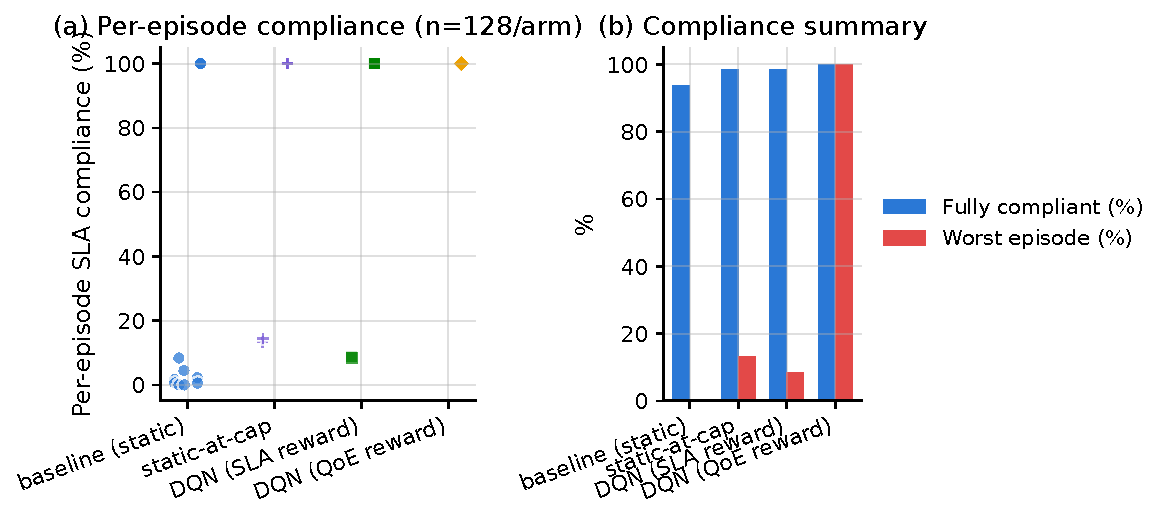
\includegraphics[width=0.76\linewidth]{figures/fig2_sla_compliance.pdf}
\caption{Per-episode SLA compliance (\%). (a) One point per episode. (b) Fraction of episodes fully SLA-compliant and worst single-episode compliance. Baseline, static-at-cap, and DQN under the SLA-only reward all show the same bimodal split; only DQN under the QoE-aware reward stays uniformly compliant.}
\label{fig:compliance}
\end{figure*}

Fig.~\ref{fig:compliance} shows this episode-by-episode: DQN under the
QoE-aware reward sits at exactly 100\% in every episode, while the
static baseline, the static-at-cap arm, and DQN under the SLA-only
reward each show the same bimodal split between fully-compliant and
collapsed episodes.

A checkpoint is a single set of frozen DQN weights saved at the end of
one offline training run; it is what is actually deployed live, making
a state-to-ceiling decision every control cycle with no further
learning. Since only one DQN-SLA checkpoint was evaluated above, we
trained 5 more independently-seeded DQN-SLA policies under the same
procedure and live-evaluated all of them at the same 21-episode
protocol. Despite converging equally well offline -- indistinguishable
Q1$\to$Q4 reward improvement across all six seeds -- live records
varied substantially (3/5 perfect, one matching the original 19/21,
one collapsing to 13/21, worse than baseline): live robustness is not
predictable from offline convergence alone, and the checkpoint above
is a representative, not best-or-worst-case, draw. This is the
practical face of the offline-environment limitation noted in
Section~III-C: two checkpoints can look equally converged offline and
still behave very differently under real traffic. This robustness
check runs each of the 6 checkpoints at 21 episodes rather than the
128-episode/arm headline protocol -- a deliberate scope cut (evaluating
6 checkpoints at 128 episodes each would cost roughly six times this
paper's entire live-evaluation budget) that is enough live rig time to
see the qualitative spread (perfect, marginal, and collapsing
checkpoints all appearing) but not enough to place a precise rate on
how often each outcome occurs; we report it as a limitation of this
check's power, not of the spread itself.

\subsection{Deployment Feasibility}
\label{sec:feasibility}
Measured directly against the real gNB, the control loop's E2
message round trip has a median latency of 0.57\,ms, and the DQN
model itself (under 20,000 parameters) selects an action in under
70\,$\mu$s on CPU. Both are a small fraction of the 5-second control
interval used in this study, indicating the learned policy adds
negligible overhead to the control loop.

Comparing offline training predictions against the live results
showed a good match for eMBB traffic, but not for URLLC and mMTC,
which were trained under a different demand assumption than what was
observed live. During this comparison we also identified a
calibration bug in Eq.~\eqref{eq:mos-form}'s inverse-throughput term
$\epsilon_k/R_k$: the environment feeds $R_k$ as a slice's PRB usage
\emph{ratio} to the gNB's total capacity, but eMBB's coefficients had
been fit assuming $R_k$ was an absolute per-UE PRB count, in the wrong
units by roughly two orders of magnitude. A real eMBB demand of
$\sim$15 PRB (ratio $\approx 0.15$) was therefore read by the log
argument as an almost-starved connection, pinning eMBB's MOS at the
scale's floor (1.0) for every observed operating point regardless of
policy quality -- understating MOS for exactly the well-served traffic
the metric is meant to reward. We refit the affected coefficients
against the ratio $R_k$ actually produced at runtime and verified the
fix directly at real observed ratios (0.05/0.15/0.24 $\to$
2.29/3.62/4.11, versus 1.00/1.00/1.00 before the fix); Table~\ref{tab:results}
above reports the resulting fully powered live re-evaluation.

\subsection{Congested Scenario (Offline)}
Sections IV-A and IV-B use one constant demand level per episode. To
test a harder, more realistic scenario, we evaluate the same trained
policies offline under continuously varying, randomised multi-slice
traffic with genuine cross-slice resource contention: when combined
demand exceeds the shared PRB pool, every slice's served allocation
is scaled down in proportion to its request, rather than each slice
being served independently. Pooled over 11 seeds (165 held-out
episodes per arm), both DQN variants raise URLLC compliance above the
static baseline's 19.7\% (to 27.7\% for the SLA-only reward, 25.0\% for
the QoE-aware reward) by actively trading off eMBB (32.7\%
$\to$7.7\%/8.2\%) and mMTC (19.8\%$\to$9.4\%/11.6\%) compliance -- the
same URLLC-first behaviour our earlier simulated work targeted
\cite{mecon-paper1,icraie-paper2}, now shown under real cross-slice
contention rather than each slice's demand being satisfied
independently, and replicating cleanly on an independent 8-seed
extension of this evaluation. Weighted by each slice's declared
priority, the static baseline still scores higher overall (24.9\% vs.\
19.1\%/17.9\% for DQN), since eMBB's importance outweighs URLLC's gain
-- a real, repeatable tradeoff whose net value depends on whether the
priority weights themselves should be revisited, an open question for
future work.

We additionally live-evaluated the same congested/URLLC-preservation
checkpoints on the real rig, at a smaller pilot scale (one seed, 2
episodes per arm). Unlike the offline result above, every arm --
including the static baseline -- was fully SLA-compliant live. This is
a scale mismatch, not a contradiction: the offline scenario's tradeoff
is driven by an imposed shared-resource-pool budget deliberately set
smaller than what the three slices' ceilings could jointly request,
whereas this rig's calibrated ceilings (summing to a small fraction of
the gNB's real 106-PRB capacity) never approach genuine physical
contention at these traffic levels, so no forced tradeoff arises live.
The QoE-aware reward nonetheless produced a materially higher URLLC
Mean Opinion Score (4.83) than the SLA-only reward (2.44) or the
static baseline (2.66) at the same 100\% compliance (pilot: 1 seed, 2
ep/arm) -- a difference in
experience quality the raw compliance numbers alone do not show. A
live reproduction of genuine physical multi-slice scarcity would
require substantially higher per-slice ceilings and traffic than this
campaign's calibration, which we leave for future work.

\subsection{Summary of Findings}
Table~\ref{tab:timeline} summarises how the live evaluation reached
its final scale: the 4-arm comparison (Table~\ref{tab:results}) grew
across three extensions of the same seed set, and the checkpoint
sensitivity check above (5 additional DQN-SLA checkpoints) is a
separate, smaller protocol run once, not a fourth extension of it.

\begin{table}[t]
\centering
\caption{Live evaluation timeline (cumulative, unless noted)}
\label{tab:timeline}
\small
\begin{tabular}{@{}p{0.1\linewidth}p{0.09\linewidth}p{0.14\linewidth}p{0.54\linewidth}@{}}
\toprule
Round & \#seeds & Ep./arm & What changed \\
\midrule
1 & 3 & 6 & Initial live 4-arm pass \\
2 & 11 & 46 & QoE-calibration issue corrected (Sec.~III-C/IV-B); first fully-powered round \\
3 & 28 & 128 & Extended for full statistical power (Table~\ref{tab:results}) \\
\midrule
\multicolumn{4}{@{}l}{\emph{Separate protocol (not additive to the above):}} \\
Robust. & 6 & 21/ckpt. & 5 extra independently-trained DQN-SLA checkpoints (Section~IV-A) \\
\bottomrule
\end{tabular}
\end{table}

At full statistical power (128 episodes/arm), the QoE-aware reward's
advantage over static control clearly holds up and is now
statistically significant against the baseline (128/128 vs.\ 126/128
for DQN-SLA and static-at-cap, 120/128 for the baseline; Fisher exact
$p=0.0070$ raw, $p=0.0209$ after Holm-Bonferroni correction across the
three vs.-baseline tests). The SLA-only reward's own edge over
static-at-cap, which a smaller-sample round suggested was a real
trade-off in the learned policy's favour, is instead a genuine null
result at full power (126/128 each, Fisher exact $p=1.0$): the two
arms are statistically indistinguishable once the sample is large
enough to say so with confidence, not merely underpowered before.
Checking 5 more independently-trained checkpoints shows part of why --
live robustness varies by training seed in a way offline convergence
does not surface. This is itself an instance of the sim-to-real
fidelity gap our systematic review's evidence-tier analysis
identifies across the field \cite{survey-paper3}: the offline training
environment's own limitations (Section~III-C) put its evidence in a
lower tier than the live result it is meant to predict, a
methodological finding about this field's evidence base as much as
about this rig specifically. The offline congested scenario still
shows URLLC prioritisation consistent with our earlier simulated work,
though not yet a net win once priorities are weighted, and does not
reproduce live at this campaign's ceiling scale -- another sim-to-real
trade-off of exactly the kind that motivates evaluating on live
hardware in the first place.

\section{Conclusion and Future Work}
This paper moved our prior simulated DRL-based slice admission control
work \cite{mecon-paper1,icraie-paper2} onto a real OAI gNB over its
native E2 control loop, radio channel still simulated. After
correcting a QoE-calibration issue, a fully powered live re-evaluation
-- extended over the course of this study to 128 episodes/arm --
showed the QoE-aware reward sustaining 100\% SLA compliance, now
significantly ahead of the static baseline (Fisher exact $p=0.0070$
raw, $p=0.0209$ Holm-adjusted for the three-way vs.-baseline family),
while the SLA-only reward and static-at-cap remained statistically
indistinguishable from each other (126/128 each -- revising our
earlier, smaller-sample finding of a significant SLA-only edge,
$p{=}0.0149\to p{=}1.0$ at full power) and only numerically, not
significantly, ahead of the static baseline's 120/128, with negligible
control-loop latency/model overhead.
An offline congested-traffic evaluation showed the learned policy can
prioritise URLLC, though not yet as a clear win once priorities are
weighted; live, no arm was forced into that tradeoff, though the
QoE-aware reward still gave URLLC a materially better experience
score.

Our future work will (1) improve the offline training environment's
temporal fidelity to real traffic, needed to make offline evaluation
predictive of live robustness rather than only a source of competent
policies (Section~III-C); (2) recalibrate ceilings and traffic to
attempt a live reproduction of genuine multi-slice physical scarcity;
and (3) extend this single-agent, single-gNB DQN -- validated live here
as the reduced-case control loop the fuller architecture sits on
(Section~I) -- toward the full GAT-MARL-FL formulation our systematic
review's own future-work directions call for \cite{survey-paper3}: a
graph-attention (GAT) topology encoder over the inter-gNB
neighbourhood, a multi-agent extension to the multi-gNB setting, and
federated learning across gNBs so policies improve without
centralising raw traffic data. That extension is our planned next
paper (\#5), building directly on the live control loop validated
here.

\section*{Acknowledgment}
This research was supported by the Ministry of Higher Education
(MOHE), Malaysia through the Fundamental Research Grant Scheme
(FRGS/1/2024/ICT06/TAYLOR/02/1).

\bibliographystyle{IEEEtran}
\bibliography{refs}

\end{document}
